%Jennifer Pan, August 2011

\documentclass[10pt,letter]{article}
	% basic article document class
	% use percent signs to make comments to yourself -- they will not show up.

\usepackage{amsmath}
\usepackage{amssymb}
	% packages that allow mathematical formatting

\usepackage{graphicx}
	% package that allows you to include graphics

\usepackage{setspace}
	% package that allows you to change spacing

\onehalfspacing
	% text become 1.5 spaced

\usepackage{fullpage}
	% package that specifies normal margins
	
\usepackage[version=3]{mhchem} % Package for chemical equation typesetting
\usepackage{graphicx} % Required for the inclusion of images
\usepackage{natbib} % Required to change bibliography style to APA
\usepackage{amsmath} % Required for some math elements 
\usepackage{booktabs}
\usepackage{floatrow}
	

\begin{document}
	% line of code telling latex that your document is beginning


\title{CS 156 Problem Set 2}

\author{Christopher Zhen}

\date{Oct 10, 2016}
	% Note: when you omit this command, the current dateis automatically included
 
\maketitle 
	% tells latex to follow your header (e.g., title, author) commands.


\section*{Problem 1}

\textbf{(B)} - The value of $\nu _{min}$ was around 0.038 in my code. This makes sense because the minimum number of heads is usually 0.

\section*{Problem 2}

\textbf{(D)} - Only these two have $\nu$ values fairly close to $\mu$. $\nu _{rand}$ was 0.501 and $\nu _{1}$ was 0.500 which are very close to $\mu = 0.5$. This makes sense because $c _{rand}$ and $c _{1}$ are pretty accurate samples of the population, but $c _{min}$ is a very skewed sample.


\section*{Problem 3} 

\textbf{(E)} - There are two possible ways to have an error: when $y = f(x)$ and $h$ gives an error or when $y \neq f(x)$ and $h = f$. The first probability is $\lambda * \mu$ and the second probability is $(1-\lambda)*(1-\mu)$.


\section*{Problem 4}

\textbf{(B)} - If $\lambda$ is $0.5$ then the expression simplifies to:

\begin{equation}
(1-0.5)*(1-\mu) + 0.5*\mu
\end{equation}
\begin{equation}
0.5*(1-\mu + \mu)
\end{equation}

\noindent Which simplifies to a probability of 0.5 and is independent of $\mu$.

\section*{Problem 5}

\textbf{(C)} - The value for $E_{in}$ obtained in my code was 0.0368 which is closest to 0.01. This means linear regression is fairly accurate for classification, but definitely not as good as PLA which makes sense.

\section*{Problem 6}

%\begin{figure}[H]
%\begin{center}
%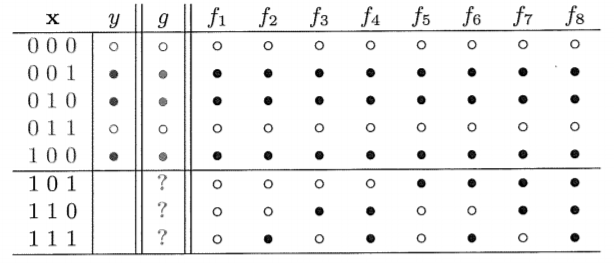
\includegraphics[width=0.75\textwidth]{FactorTable.PNG}
%\caption{Table courtesy of the textbook \textit{Learning from Data}.}
%\label{FactorTable}
%\end{center}
%\end{figure}

\textbf{(C)} - This time, $E_{out}$ was calculated to be 0.0419 which is closest to 0.01. This is slightly higher than $E_{in}$ since this is not the data set we learned from, but it's also pretty low since the algorithm should do an okay job of learning f.

\section*{Problem 7}

\textbf{(A)} - When using the w determined from linear regression, PLA typically takes 4.811 iterations to converge. This makes sense because without using linear regresion, PLA takes around 10-15 iterations to converge with 10 data points, so it should be considerably less if the initial guess is almost right.

\section*{Problem 8}

\textbf{(D)} - My code returned a value of $E_{in}$ of 0.5128 which is closest to 0.5. This makes sense because we're trying to use a linear model to classify non-linear data so it'll probably result in a really bad fit.

\section*{Problem 9}

\textbf{(A)} - The value of $\tilde{w}$ from the code was: [-1.01, 0.004, -0.003, -0.004, 1.59, 1.58]. This result was obtained by averaging 1000 iterations of linear regression and is most similar to answer choice A. This choice also makes sense because it is fairly close to the target function (which would be [-0.6, 0, 0, 0, 1, 1]).

\section*{Problem 10}

\textbf{(B)} - My code calculated $E_{out}$ to be 0.0753 which is pretty close to 0.1. $E_{in}$ was found to be around 0.0566. This is pretty impressive because it represents a significant increase over the original linear fitting algorithm.

\end{document}
	% line of code telling latex that your document is ending. If you leave this out, you'll get an error
